	\section{Network-Setup}
	The setup of the iCTF 2015 is shown in the graphic \ref{img:setup}. The Router has a private VPN running, tunneling all traffic through the THI-Network. Also the Router creates 2 sub-networks. The "bad network" (shown in red) holds the iCTF-Router and vulnerable VM, as well as some attacker PCs, which will run the exploits against other teams. In the "good network" (shown in green) are the participants, who have a local copy of the vulnerable Image and develop patches and exploit. It's to mention, that the router has ip-tables-rules specified, so the "bad network" can not communicate with the "good network". Also, the Attacker-PCs have to route their traffic through the CTF-Router. This should be solved differently in the upcoming CTFs, since the separation of the 2 networks needed a lot of time to be configured.
	\begin{figure}
		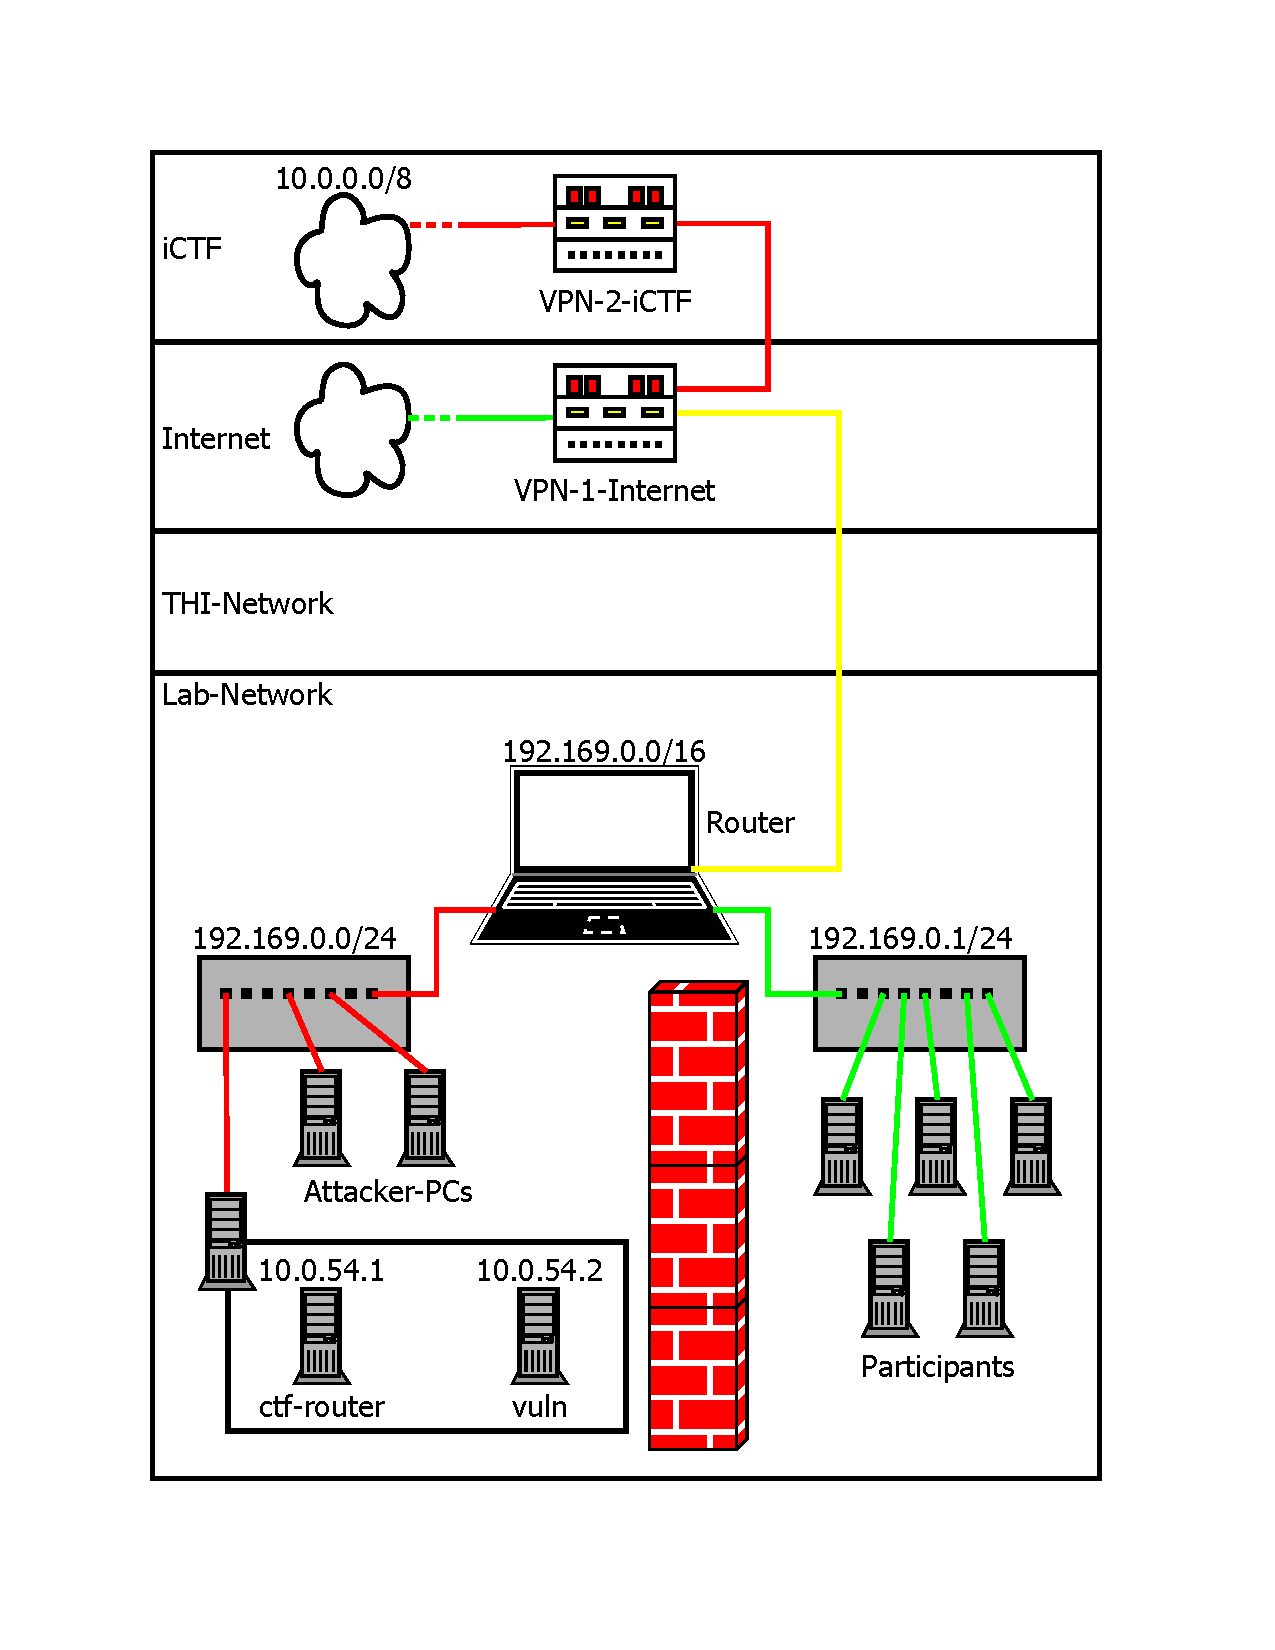
\includegraphics[width=\textwidth]{images/setup.pdf}
		\caption{Network-Setup iCTF 2015}
	\end{figure}
	%Dungeon Service
	\label{img:setup}